%!TEX root = aaai2014.tex
\section{PLANNING UNDER UNCERTAINTY}
\label{sec:planning}

% After several interaction with the user, our algorithm is able to identify a task among a set of possible tasks. To do so it has to explore regions that allow to disambiguate among hypothesis. There are several efficient model-based reinforcement learning exploration methods that add an exploration bonus for states that might provide more learning gains. Several theoretical results show that these approaches allow to learn tasks efficiently \cite{brafman2003r,kolter2009near}. We define an uncertainty measure and use model-based planning to select sequences of actions that guide the agent toward states that better identify the desired task.

To solve our problem we need to identify simultaneously the task and how to interpret teaching signals. To do so the system has to explore regions that allow to disambiguate among hypothesis. There are several efficient model-based reinforcement learning exploration methods that add an exploration bonus for states that might provide more learning gains. Several theoretical results show that these approaches allow to learn tasks efficiently \cite{brafman2003r,kolter2009near}. We define an uncertainty measure and use model-based planning to select sequences of actions that guide the agent toward states that better identify the desired task.

In order to exemplify the specificity of our problem in terms of planning we present a simple experiment and compare the effect of different action selection strategies. In this scenario, the agent is in a T world with 7 states and can perform 4 actions (right, left, up, and down). The user wants the robot to reach the left edge (marked by G1) of the T, (see Figure~\ref{fig:planningExplained} top). The agent knows the users wants it to go to one of the two edges (G1 or G2) but not which one. The agent will perform some actions, and the user will assess the correctness of each agent's action by providing a two dimensional teaching signal. The agent does not known which signal means ``correct'' and which signal means ``incorrect''. As there is two possible tasks, the agent will assign labels to every user's signals according to each hypothesis. The result of the labeling process is displayed as colored dots (green for ``correct''and red for ``incorrect'') in Figure \ref{fig:planningExplained} (a, b, and c), where the left part corresponds to hypothesis 1 (G1) and the right part to hypothesis 2 (G2).

 % The goal of the agent is to reach one of the two edges of the T world (see figure \ref{fig:planningExplained} top), the one the user has in mind. After each agent's move, the user assesses the correctness of the agent action by providing a two dimensional teaching signal. 

\begin{figure}[!ht]
  \centering
      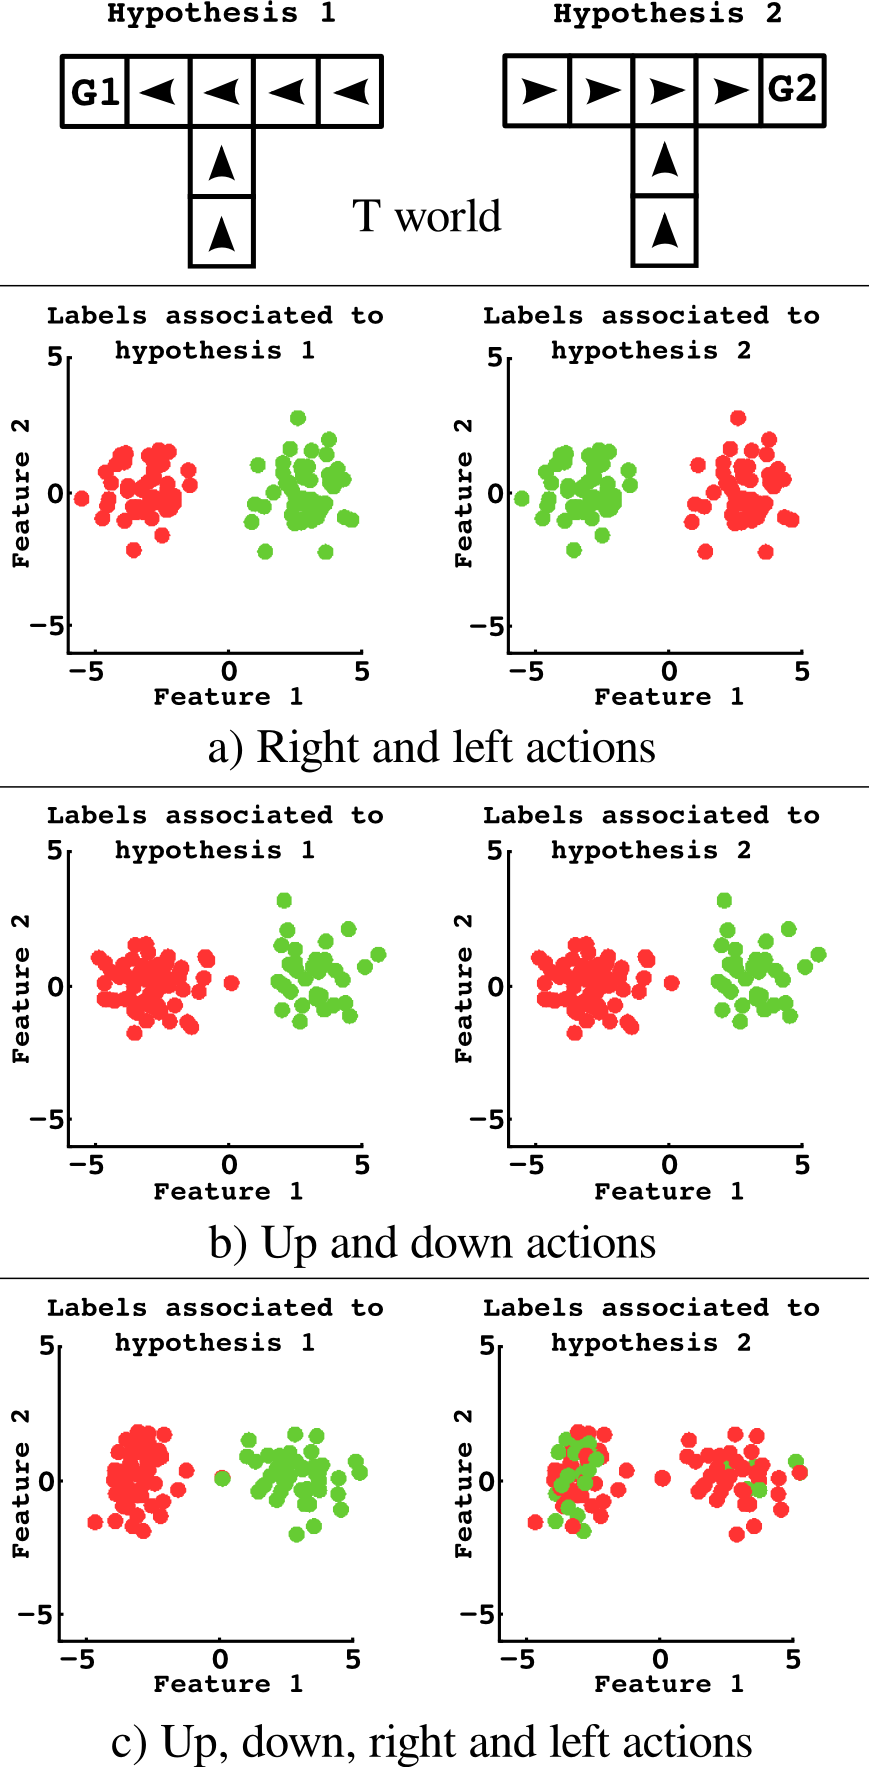
\includegraphics[width=0.93\columnwidth]{img/planning.png}
      \caption{A ``T world'' scenario and the interpretation results for different planning strategies. The agent knows it should reach either of the two edges of the T world (marked with the letter G). The arrows represent the optimal policy. For each move the agent receives an unlabeled two dimensional teaching signal, corresponding to user's assessments on the agent's actions. The teacher's goal is to have the agent reach G1. As the agent do not have access to this information, it interprets the signal according to each hypothesis (G1 and G2). a) shows the interpretation results if the agent only perform right and left actions in the top of the T world, b) shows the interpretation results when the agent only performs up and down actions in the trunk of the T, and c) shows the interpretation results for an agent performing all possible actions. Only the method c) allow to differentiate between hypothesis.}
    \label{fig:planningExplained}
\end{figure}

If the agent knew how to interpret the signal, i.e. which signal corresponds to correct or incorrect feedback, the optimal action to differentiate between the two hypothesis would be to perform right and left actions in the top part of the T. However in our problem the classifier is not given and the agent is building a different model for each hypothesis. As a results, we end up with two opposite interpretations of the user signal, which are both as valid (see Figure~\ref{fig:planningExplained}a) and do not allow to differentiate between hypothesis.

Considering that the agent does not know the signal to meaning classifier, a sensitive option is to select actions that allow to unequivocally identify the model. In our scenario taking only up and down actions in the trunk of the T leads to identical interpretation for each hypothesis (see Figure~\ref{fig:planningExplained}b). However this method do not allow to disambiguate between hypothesis and in most setting, such as the grid world we consider later, there is no state-action pair leading to unequivocal interpretations.

However performing all the four actions allow to disambiguate between hypothesis. As shown in Figure~\ref{fig:planningExplained}c, hypothesis 1 stands out by the nice coherence between the labels and the spacial organization of the data. This informs us that hypothesis 1 is the task the user has in mind and that feedback signals in the right and left part of the feature space means ``correct'' and ``incorrect'' respectively.

For our kind of problem the agent can not just try to differentiate hypothesis by finding state-action pair where expected feedback differs but should also collect data to build a good model or at least invalidate other models. Can we find a measure of uncertainty that account for both? Going back to Figure~\ref{fig:planningExplained} (a and b), we understand that, to differentiate hypothesis in situation a) the best actions to perform are up and down in the T trunk while in situation b) the best actions to perform are right and left in the top part of the T. This corresponds to the uncertainty in the signal space. In the case of a) when going left both hypothesis agree that they will receive a signal in the right part of the feature space even if they disagree on its meaning. However for action down, both hypothesis agree they should receive a signal of meaning ``incorrect'' but disagree on the expected location of such signal in the feature space. In the case of b) when going up both hypothesis agree they will receive a signal in the right part of the feature space and agree on its meaning. However for action left, both hypothesis disagree about the meaning of the signal they should receive and as both share the same signal model they expect a signal in different locations of the feature space.

Estimating uncertainty in the signal space is in practice too costly as it requires to compute, for every state-action pair, the overlap between many continuous probability distributions weighted by their respective expected contribution. Following the discussion presented in previous section, we will rely on our pseudo-likelihood metric. As we cannot predict, neither control, the signal we will receive for a particular state-action, we will rely on our past history of signal and compute the expected joint probability based on previously experienced signals.

% \todo{transition with actual equations, uncertainty in signal space is too costly to compute. We therefore rely on an approximation, projecting back signal space into some sort of expected meaning space and comparing with theoretical meaning space, i.e. the probability that expected labels $l^{H^{\xi_t}}$ equals predicted labels $l^{H^{\theta_{i}^{\xi_t}}}$}

% \todo{the following explanation was quite intuitive with respect to previous algo version but did not cover the details that I tried to explain above}

% To differentiate between tasks, our algorithm computes the probability that expected labels $l^{\xi_t}$ equals predicted labels $l^{\theta^{\xi_t}}$. In order to find which task is the correct one, we need to explore the state space where this value differs between likely hypothesis. As we cannot predict, neither control, the signal we will receive for a particular state-action, we will rely on our past history of signal and compute the expected joint probability based on previously experienced signals.

We note:
\begin{eqnarray}
J^{\xi_t}(s,a,e) = \sum_{l_c}\sum_l  p(e | l_c, \theta)  p(l_c | l, \theta) p(l|s,a,\xi_t) \nonumber
\end{eqnarray}
which is Eq.~\ref{eq:pseudo2} for only one new expected observation $e$, so the product over iterations disappears. And $J^{\xi}(s,a,e)$ the vector $[J^{\xi_1}(s,a,e), \ldots, J^{\xi_T}(s,a,e)]$.

The uncertainty of one state-action pair given a signal $e$ is computed as the weighted variance of the joint probability predictions with weights $W^{\xi} = [W^{\xi_1}, \ldots, W^{\xi_T}]$ (see Eq.~\ref{eq:weight}):
\begin{eqnarray}
U(s,a|e) = weightedVariance(J^{\xi}(s,a,e), W^{\xi})
\label{eq:planningOneSignal}
\end{eqnarray}

The uncertainty for a state-action pair is given by:
\begin{eqnarray}
U(s,a) & = & \int_{e} U(s,a|e) p(e) de
\end{eqnarray}
which we approximate by summing values of $U(s,a|e)$ for different signals $e$:
\begin{eqnarray}
U(s,a) & \approx & \sum_{e} U(s,a|e) p(e)
\label{eq:planning}
\end{eqnarray}
with $p(e)$ assumed uniform.
%

% Finally, we evaluate $U(s,a)$ by summing values of $U(s,a|e)$ for different signals $e$:
% \begin{eqnarray}
% U(s,a) & = & \int_{e} U(s,a|e) p(e) de \nonumber \\
% 		 & \propto & \sum_{e} U(s,a|e) p(e)
% \label{eq:planning}
% \end{eqnarray}

Our measure of global uncertainty $U(s,a)$ will be higher when, for a given state-action there is a high incongruity of expectation between each hypothesis and according to each hypothesis current probability. 

This measure is then used as a classical exploration bonus method. We will switch to a pure exploitation of the task after reaching the desired confidence level.

Interestingly this approach generalizes over other active sampling method \cite{lopes2009active}, if the classifier is known, equation \ref{eq:planningOneSignal} reduces to the one presented in \cite{macl11simul} and is no longer dependent on signal $e$. As our uncertainty function combines uncertainty on both signal and task space, when the former is known, the latter becomes the sole source of ambiguity.


% Our goal is to learn which task $\xi$ among a set of possible task $\xi_1,\ldots,\xi_T$ is the one taugh by the trainer. To do so we compute the cumulative probability that expected labels ($l_{i+1}^{\xi_t}$) equals predicted labels ($l_{i+1}^{U_t}$). In order to find which task is the correct one, we need to explore the space such that the expected joint probability between likely hypothesis differs.

% with weighted variance define as: \todo{cite if needed}
% \begin{eqnarray}
% wVar(x,w) = \frac{\sum_{i=1}^n w_i}{(\sum_{i=1}^n w_i)^2-(\sum_{i=1}^n {w_i^2})} \sum_{i=1}^N w_i \left(x_i - \bar{x}^*\right)^2
% \end{eqnarray}
% where: $\bar{x}^* = \frac{\sum_{i=1}^n w_i x_i}{\sum_{i=1}^n w_i}$

%Only the relative value of $U(s,a)$ matters and the use of variance is arbitrary, any function having similar properties of measuring variation between estimates would do.


% We note $J_{i}^{\xi}(s,a,e) = [J_{i}^{\xi_1}(s,a,e), \ldots, J_{i}^{\xi_T}(s,a,e)]$
%  % with:
% % \begin{eqnarray}
% % J_{i}^{\xi_t}(s,a,e) = \sum_{l} p(l^H^{\xi_t}} = l | s, a, \xi_t) p(l^H^{\theta_i^{\xi_t}}} = l | e, \theta_i^{\xi_t} )
% % \end{eqnarray}
% the vector of probability that the label $l^H^{\xi_t}}$ expected from the task $\xi_t$ equals the label $l^H^{\theta_i^{\xi_t}}}$ predicted by the classifier $\theta_i^{\xi_t}$ for each task. We define $W_{i}^{\xi} = [W_{i}^{\xi_1}, \ldots, W_{i}^{\xi_T}]$ with $W_{i}^{\xi_t}$ the minimum pairwise normalized likelihood of hypothesis $\xi_t$ at iteration $i$, see eq. \ref{eq:weight}.